\documentclass[a4paper, 12pt]{article}

% \usepackage[utf8]{inputenc}
% \usepackage{tgtermes}
% \usepackage{fouriernc}
\usepackage[T1]{fontenc}
\usepackage[margin=3cm]{geometry}
\usepackage{babel}

\usepackage{biblatex}
\addbibresource{refs.bib}

\usepackage{amssymb}
\usepackage{amsmath}

\usepackage{ebproof}

\usepackage{enumerate}
\usepackage{verbatim}

\usepackage{xcolor}

\usepackage{listings}
\lstset{mathescape=true,
 xleftmargin=.25in}
\usepackage{quiver}

\usepackage[ruled]{algorithm2e}
\SetKwInput{Input}{\sc Input}
\SetKwInput{Output}{\sc Output}

\usepackage[skip=10pt]{parskip}

\newcommand{\N}{\mathbb{N}}
\newcommand{\Z}{\mathbb{Z}}
\newcommand{\Q}{\mathbb{Q}}
\newcommand{\R}{\mathbb{R}}
\newcommand{\C}{\mathbb{C}}
\newcommand{\B}{\mathbb{B}}
\newcommand{\dif}{\mathrm{d}}
\DeclareMathOperator{\Arg}{Arg}
\DeclareMathOperator{\IN}{IN}
\DeclareMathOperator{\LT}{lt}
\DeclareMathOperator{\LM}{lm}
\DeclareMathOperator{\LC}{lc}
\DeclareMathOperator{\lcm}{lcm}
\newcommand{\la}[1]{\lambda{#1}.\,}


% Kan Danny godt lide
\usepackage[autostyle]{csquotes}
% \usepackage{kpfonts}
% \usepackage{inconsolata}
\linespread{1.06}

% \usepackage{minted}
% \usemintedstyle{tango}
% \setminted{fontsize=\footnotesize}
% \setminted{breaklines}
% \newcommand{\lean}[1]{\mintinline{lean}{#1}}

\usepackage{fontspec}
% \setmonofont{JuliaMono}
% \setmainfont{Linux Libertine O}
% \setmathfont[Digits, Latin]{Linux Biolinum O}
\usepackage{libertinus}
% \usepackage{ebgaramond-maths}
% \usepackage{ebgaramond}
% \usepackage[cmintegrals, cmbraces]{newtxmath}

\usepackage{xcolor}
\usepackage{hyperref}
\hypersetup{%
	pdftitle=Parametric Gröbner bases,
	pdfauthor={Andreas Bøgh Poulsen},
	colorlinks,
	linkcolor={red!50!black},
	citecolor={red!50!black},
	urlcolor={red!50!black},
	bookmarksnumbered=true
}

\usepackage[ntheorem]{mdframed}
\usepackage[amsmath,thmmarks,hyperref]{ntheorem}
\usepackage[capitalize]{cleveref}

% Frame for theorems
\definecolor{shadecolor}{gray}{0.93}
\definecolor{rulecolor}{gray}{0.4}
\mdfdefinestyle{thmframed}{%
	%usetwoside=false, % For use with memoir twoside
	skipabove=0.5em plus 0.4em minus 0.2em,
	skipbelow=0.5em plus 0.4em minus 0.2em,
	leftmargin=-7pt, rightmargin=-7pt, innerleftmargin=6pt,
	innerrightmargin=6pt, innertopmargin=6pt, innerbottommargin=3pt,
	% linewidth=1pt, linecolor=rulecolor, backgroundcolor=shadecolor,
  linewidth=1.5pt, linecolor=rulecolor, topline=false, bottomline=false, rightline=false, %leftmargin=1em,
	splittopskip=1.2em minus 0.2em,
	splitbottomskip=0.5em plus 0.2em minus 0.1em,
}
\mdfdefinestyle{thmempty}{
  usetwoside=false, % For use with memoir twoside
	skipabove=0.5em plus 0.4em minus 0.2em,
	skipbelow=0.5em plus 0.4em minus 0.2em,
	leftmargin=-7pt, rightmargin=-7pt, innerleftmargin=6pt,
	innerrightmargin=6pt, innertopmargin=6pt, innerbottommargin=3pt,
	% linewidth=1pt, linecolor=rulecolor, backgroundcolor=shadecolor,
  linewidth=1.5pt, linecolor=rulecolor, topline=false, bottomline=false, rightline=false,
	splittopskip=1.2em minus 0.2em,
	splitbottomskip=0.5em plus 0.2em minus 0.1em,
}

% New theorem style with a dot
\makeatletter
\newtheoremstyle{changedot}%
  {\item[\hskip\labelsep \theorem@headerfont ##2~~$\cdot$~~##1\theorem@separator]}%
  {\item[\hskip\labelsep \theorem@headerfont ##2~~$\cdot$~~##1\ (##3)\theorem@separator]}

\newtheoremstyle{changedotbreak}%
  {\item\hbox to \textwidth{\theorem@headerfont ##2~~$\cdot$~~##1\theorem@separator\hfill}}%
  {\item\hbox to \textwidth{\theorem@headerfont ##2~~$\cdot$~~##1\
      (##3)\theorem@separator\hfill}}
\makeatother

\theoremstyle{changedot}
\theoremseparator{.}
% \newmdtheoremenv[style=thmframed]{theorem}{Theorem}[section]
% \newmdtheoremenv[style=thmframed]{proposition}[theorem]{Proposition}
% \newmdtheoremenv[style=thmframed]{lemma}[theorem]{Lemma}
% \newmdtheoremenv[style=thmframed]{corollary}[theorem]{Corollary}
\newmdtheoremenv[style=thmempty]{theorem}{Theorem}[section]
\newmdtheoremenv[style=thmempty]{proposition}[theorem]{Proposition}
\newmdtheoremenv[style=thmempty]{lemma}[theorem]{Lemma}
\newmdtheoremenv[style=thmempty]{corollary}[theorem]{Corollary}
\newmdtheoremenv[style=thmempty]{example}[theorem]{Example}

\theorembodyfont{\normalfont}
%\theoremsymbol{\ensuremath{\triangle}}
\newmdtheoremenv[style=thmframed]{definition}[theorem]{Definition}

\theoremstyle{changedotbreak}
\newmdtheoremenv[style=thmframed]{definitionbreak}[theorem]{Definition}

\theoremstyle{nonumberplain}
\theoremheaderfont{\normalfont\itshape}
\theorembodyfont{\normalfont}
\theoremsymbol{\ensuremath{\square}}
\newtheorem{proof}{Proof}

\Crefname{theorem}{Theorem}{Theorems}
\Crefname{proposition}{Proposition}{Propositions}
\Crefname{lemma}{Lemma}{Lemmata}
\Crefname{corollary}{Corollary}{Corollaries}
\Crefname{definition}{Definition}{Definitions}

\crefformat{equation}{(#2#1#3)}

% / Kan Danny godt lide

% \usepackage[eng,exjobb]{KTHEEtitlepage}

\title{Parametric Gröbner bases\\{\large \textsc{Geometry \& applications}}}
\author{Andreas Bøgh Poulsen, student id: 201805425}

\newcommand*{\titleGM}{%\begingroup % Create the command for including the title page in the document
%\hbox{ % Horizontal box
\hspace*{0.2\textwidth} % Whitespace to the left of the title page
\rule{1pt}{\textheight} % Vertical line
\hspace*{0.05\textwidth} % Whitespace between the vertical line and title page text
\parbox[b]{0.75\textwidth}{ % Paragraph box which restricts text to less than the width of the page
{\noindent\Huge\bfseries  Parametric Gröbner bases\\{\large \textsc{Geometry \& applications}}\\}\\[2\baselineskip] % Title
{\large \textit{Andreas Bøgh Poulsen \hfill \oldstylenums{201805425} }}\\%[1\baselineskip]
% {\large  } \\[4\baselineskip] % Tagline or further description
{\large } % Author name
\parbox[b][0pt]{0.5\textwidth}{
  \hspace{2cm}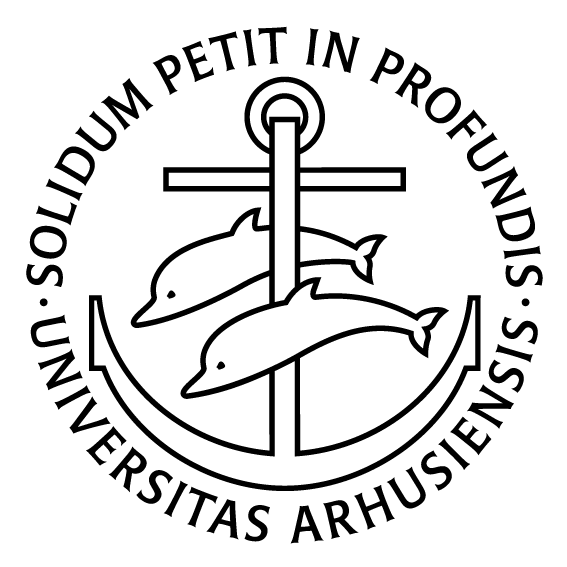
\includegraphics[width=0.5\textwidth]{ausegl_sort.png}
  \vspace{-10cm}
}

% \begin{centering}
  % 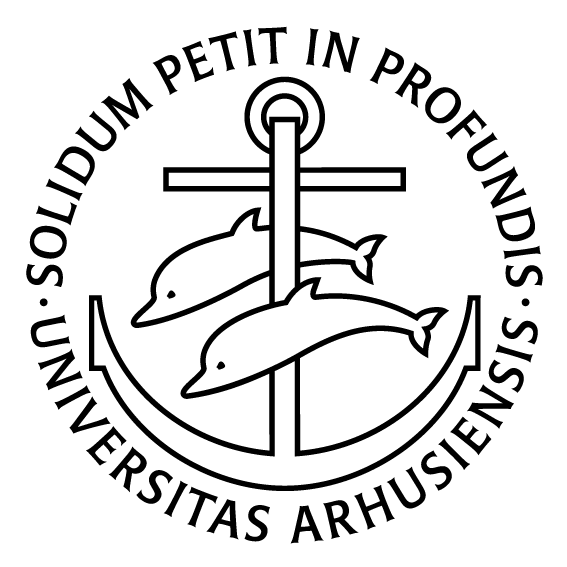
\includegraphics[width=0.5\textwidth]{ausegl_sort.png}
% \end{centering}
\vspace{0.5\textheight} % Whitespace between the title block and the publisher
\vfill
{\noindent Supervisor: Niels Lauritzen \hspace{2.5cm} 
\includegraphics{AU_logo.png}  }\\[\baselineskip] % Publisher and logo
}%}
% \endgroup
}

\begin{document}
% \maketitle
\pagenumbering{roman}
\titleGM
% \vfill
% Vejleder: Niels Lauritzen
% \strut\hfill
% 
\includegraphics[right]{AU_logo.png}
\newpage
\tableofcontents

\newpage
\pagenumbering{arabic}

\section*{Introduction}


\section{Preliminaries}
This project will assume familiarity with ring theory, multivariate polynomials over fields. A familiarity with Gröbner bases will be beneficial, but we will introduce the necesary notations and definitions. Let $R$ be a Noetherian, commutative ring and $X = (x_{1}, x_{2}, \dots, x_{n})$ be an ordered collection of symbols. We denote the ring of polynomials in these variables $R[X]$. Given two (disjoint) sets of variables $X$ and $Y$, we will use $R[X, Y]$ to mean $R[X \cup Y]$, which is isomorphic to $R[X][Y]$. A monomial is a product of variables and a term is a monomial times a coefficient. We denote a monomial as $X^{v}$ for some $v \in \N^{n}$.

\begin{definition}[Monomial order, leading term]
  A \textit{monomial order} is a total order $<$ on the set of monomials satisfying that $u < v \implies wu < wv$.

  Given a monomial order $<$ and a polynomial $f \in R[X]$, the \textit{leading term} of $f$ is the term with the largest monomial w.r.t. $<$ and is denoted by $\LT_{<}(f)$. If $\LT_{<}(f) = a\cdot m$ for some monomial $m$ and $a \in R$, then we denote $\LM_{<}(f) = m$ and $\LC_{<}(f) = a$. If $<$ is clear from context, it will be omitted.
\end{definition}

These definitions naturally extend to sets of polynomials, so given a set of polynomials $F \subset k[X]$, we denote $\LM_{<}(F) := \{\LM_{<}(f) \mid f \in F\}$. The above definitions work over a general ring (and we will use that), for from here, we'll work over a field $k$. With this, we can give the definition of a Gröbner basis.

\begin{definition}[Gröbner basis]
  Let $G \subset k[X]$ be a finite set of polynomials and $<$ be a monomial order. We say $G$ is a \textit{Gröbner basis} if
  $\langle \LT_{<}(G) \rangle = \langle \LT_{<}(\langle G \rangle ) \rangle $.
\end{definition}

\section{Definitions and initial results}
The purpose of this project is to study parametric Gröbner bases, so let's introduce those. The bare concept is rather simple.

\begin{definition}[Parametric Gröbner basis]\label{def:par_grb}
  Let $k$, $k_{1}$ be fields, $U$ and $X$ be collections of variables and $F \subset k[X, U]$ be a finite set of polynomials. A \textit{parametric Gröbner basis} is a finite set of polynomials $G \subset k[X, U]$ such that $\sigma(G)$ is a Gröbner basis of $\langle \sigma(F) \rangle$ for any ring homomorphism $\sigma : k[U] \to k_{1}$.
\end{definition}

We call such a $\sigma : k[U] \to k_{1}$ a \textit{specialization}. By the linearity of $\sigma$, all such ring homomorphisms can be characterized by their image of $U$. Thus, we can identify $\{\sigma : k[U] \to k_{1} \mid \sigma \text{ is a ring hom.}\}$ with the affine space $k_{1}^{m}$ when $U$ has $m$ elements. For $\alpha \in k_{1}^{m}$ we'll denote the corresponding map
\[\sigma_{\alpha}(u_{i}) = \alpha_{i} \quad \text{for $u_{i} \in U$}\] extended linearly.

When we work with these parametric Gröbner bases, it will be more convenient to have a bit more information attached to them, namely which elements are required for which $\sigma$. Since $\sigma$ is described by an $\alpha \in k_{1}^{m}$, we can restrict them using subsets of $k_{1}^{m}$.

\begin{definition}[Vanishing sets \& algebraic sets]
  Let $E$ be a finite subset of $k[X]$. Then the \textit{vanishing set} of $E$ is $V(E) := \{v \in k^{n} \mid e(v) = 0 \;\; \forall e \in E\}$.

  An \textit{algebraic set} is a set of the form $V(E) \setminus V(N)$ for two finite subsets $E$ and $N$ of $k[X]$.
\end{definition}

\begin{definition}[Gröbner system]
  Let $A$ be an algebraic set and $F, G \subset k[X, U]$ be finite sets. Then $(A, G)$ is called a \textit{segment of a Gröbner system for $F$} if $\sigma_{\alpha}(G)$ is a Gröbner basis of $\langle \sigma_{\alpha}(F) \rangle$ for all $\alpha \in A$. A set $\{(A_{1}, G_{1}), \dots, (A_{t}, G_{t})\}$ is called a \textit{Gröbner system} if each $(A_{i}, G_{i})$ is a segment of a Gröbner system. A Gröbner system $\{(A_{1}, G_{1}, \dots, (A_{t}, G_{t}))\}$ is called \textit{comprehensive}, if $\bigcup_{i=1}^{t}A_{i} = k_{1}^{|U|}$. We also say a Gröbner system is \textit{comprehensive on $L \subset k_{1}^{|U|}$} if $\bigcup_{i=1}^{t}A_{i} = L$.
\end{definition}

We will sometimes call a triple $(E, N, G)$ for a segment of a Gröbner system. By this we mean that $(V(E) \setminus V(N), G)$ is a segment of a Gröbner system.

\begin{example}
  Let $X = \{x, y\}$ and $U = \{u\}$ and consider the polynomials $f(x, y, u) = ux^{2} + x$ and $g(x, y, u) = xy + 1$. When $u \neq 0$, a Gröbner basis of $\langle f, g \rangle$ could be $(y-u, ux + 1)$, whatever $u$ may be. \colorbox{red}{TODO}
\end{example}

\colorbox{red}{Skriv om Kalkbrener}
\begin{definition}[Leading coefficient w.r.t.\ variables]
  Let $f \in k[U][X]$. Then the leading term of $f$ is denoted $\LT_{U}(f)$, the leading coefficient is $\LC_{U}(f)$ and the leading monomial is $\LM_{U}(f)$. These notations are also used when $f \in k[X, U]$, just viewing $f$ as a polynomial in $k[U][X]$.
\end{definition}

Note that $\LC_{U}(f) \in k[U]$, i.e.\ the leading term is a polynomial in $k[U]$ times a monomial in $X$.

From this point, we assume that the monomial order on $k[X, U]$ satisfies $X^{v_{1}} > U^{v_{2}}$ for all $v_{1} \in \N^{|X|}$ and $v_{2} \in \N^{|U|}$. This monomial order restricts to a monomial order on $k[X]$, denoted by $<_{X}$. Note that this assumption is not too restrictive, as we're usually only interested in a certain monomial order on the variables, since the parameters will be specialized away anyway. Thus for a given monomial order $<_{X}$, we can construct a suitable monomial order on $k[X, U]$, by using $<_{X}$ and breaking ties with any monomial order on $k[U]$.

\subsection{A useful criterion}
In this section we will prove a criterion to decide when a Gröbner basis $G$ of an ideal $\langle F \rangle$ maps to a Gröbner basis $\sigma(G)$ if the ideal $\langle \sigma(F) \rangle$. This is theorem 3.1 in \cite{Kalkbrener}.

\begin{lemma}\label{lem:grb_iff_reduc_to_z}
  Let $G$ be a Gröbner basis of an ideal $\langle F \rangle$ w.r.t. $<$, let $\sigma : k[U] \to k_{1}$ be a specialization and set $G_{\sigma} = \{\sigma(g) \in G \mid \sigma(\LC_{U}(g)) \neq 0\} = \{g_{1}, g_{2}, \dots, g_{l}\} \subset k_{1}[X]$. Then $G_{\sigma}$ is a Gröbner basis of the ideal $\langle \sigma(F) \rangle$ w.r.t. $<_{X}$ if and only if $\sigma(g)$ is reducible to 0 modulo $G_{\sigma}$ for every $g \in G$.
\end{lemma}
\begin{proof}
  First, we prove ``$\implies$'': Suppose $G_{\sigma}$ is a Gröbner basis of $\langle \sigma(F) \rangle$. Since $\sigma$ is linear and every element of $\langle F \rangle$ is a linear combination of elements in $F$, we have $\langle \sigma(F) \rangle = \sigma(\langle F \rangle)$. Since $g \in F$ for every $g \in G$, $\sigma(g) \in \langle \sigma(F) \rangle$, thus $\sigma(g)$ reduces to 0 modulo $G_{\sigma}$.

  Next, we prove ``$\Longleftarrow$'': Assume that $\sigma(g)$ is reducible to 0 modulo $G_{\sigma}$ for every $g \in G$ and let $f \in \langle F \rangle$ such that $\sigma(f) \neq 0$. It's enough to show that there exists a $g \in \langle F \rangle$ such that $\LM_{U}(g) \mid \LM_{U}(\sigma(f))$ and $\sigma(\LC_{U}(g)) \neq 0$. Indeed, if that is the case, then $\LT(\sigma(g))$
\end{proof}

\subsection{Computing Gröbner systems}
We will use lemma~\ref{lem:grb_iff_reduc_to_z} in a slightly different formulation:

% \begin{lemma}
%   Let $G = \{g_{1}, g_{2}, \dots, g_{k}\}$ be a Gröbner basis of an ideal $\langle F \rangle$ in $k[X, U]$ w.r.t $<$ and let $\alpha \in V(G \cap k[U])$. If $\sigma_{\alpha}(\LC_{U}(g)) \neq 0$ for each $g \in G \setminus (G \cap k[U])$, then $\sigma_{\alpha}(G)$ is a Gröbner basis of $\langle \sigma_{\alpha}(F) \rangle$.
% \end{lemma}
% \begin{proof}
%   Since $\alpha \in V(G \cap k[U])$ and $\LC_{U}(g) = g$ for any $g \in G \cap k[U]$, we have that $\sigma_{\alpha}(\LC_{U}(g)) = 0$ for all $g \in G \cap K[U]$. By assumption, $\sigma_{\alpha}(\LC_{U}(g)) \neq 0$ for any $g \notin G \cap k[U]$, thus $\sigma_{\alpha}(\LC_{U}(g)) = 0 \iff g \in G \cap k[U] \iff \sigma_{\alpha}(g) = 0$.

%   Now, $G_{\alpha} = \{\sigma_{\alpha}(g) \mid \sigma_{\alpha}(\LC_{U}(g)) \neq 0\}$ and take any $g \in G$. If $\sigma_{\alpha}(g) \in G_{\alpha}$, then $\LT(\sigma_{\alpha}(g)) = \sigma_{\alpha}(\LC_{U}(g)) \cdot \LM_{U}(g)$ since $x > u$ for all $x \in X$ and $u \in U$. Thus, $\sigma_{\alpha}(g)$ is reducible to $0$ modulo $G_{\alpha}$, since it's leading term is divisible by its own leading term.  On the other hand, if $\sigma_{\alpha}(g) \notin G_{\alpha}$, then $\sigma_{\alpha}(g) = 0$, so is immediately reducible to zero.
% \end{proof}


\begin{lemma}\label{lem:grb_if_nmap_to_z}
  Let $G = \{g_{1}, g_{2}, \dots, g_{k}\}$ be a Gröbner basis of an ideal $\langle F \rangle$ in $k[X, U]$ w.r.t $<$ and let $\alpha \in k_{1}^{m}$. If $\sigma_{\alpha}(\LC_{U}(g)) \neq 0$ for each $g \in G \setminus (G \cap k[U])$, then $\sigma_{\alpha}(G)$ is a Gröbner basis of $\langle \sigma_{\alpha}(F) \rangle$.
\end{lemma}
\begin{proof}
  Let $G_{\alpha} = \{\sigma_{\alpha}(g) \mid \sigma_{\alpha}(\LC_{U}(g)) \neq 0\}$. If there is any $g \in G$, such that $\sigma_{\alpha}(g) \in k_{1} \setminus \{0\}$, then $g \in G \cap k[U]$ since $\sigma_{\alpha}(\LC_{U}(g)) \neq 0$ for all $g \in G \setminus K[U]$. Furthermore, since $g \in \langle F \rangle$, we get that $\langle \sigma_{\alpha}(F) \rangle = k_{1}[X]$ and $\sigma_{\alpha}(G)$ is a Gröbner basis.

  If there is no such $g$, then $\alpha \in V(G \cap k[U])$. Take any $g \in G$. If $\sigma_{\alpha}(g) \in G_{\alpha}$, then $\LT(\sigma_{\alpha}(g)) = a \cdot \LM_{U}(g)$ for some $a \in k_{1}$ since $X^{v_{1}} > U^{v_{2}}$. Thus the monomial of its leading term is preserved by $\sigma_{\alpha}$, so $\sigma_{\alpha}(g)$ is reducible to $0$ modulo $G_{\alpha}$, since it's leading term is divisible by its own leading term.

  On the other hand, if $\sigma_{\alpha}(g) \notin G_{\alpha}$, then we must have $g \in G \cap k[U]$. Since $\alpha \in V(G \cap k[U])$ then $\sigma_{\alpha}(g) = 0$, so is immediately reducible to zero. Thus $\sigma_{\alpha}(G)$ is a Gröbner basis of $\langle \sigma_{\alpha}(F) \rangle$ by lemma~\ref{lem:grb_iff_reduc_to_z}.
\end{proof}

With lemma~\ref{lem:grb_iff_reduc_to_z} in mind, we can start constructing Gröbner systems. Let $G$ be a reduced Gröbner basis of an ideal $\langle F \rangle \subset k[X, U]$, and let $H = \{\LC_{U}(g) \mid g \in G \setminus k[U]\}$. Then $\left(k_{1}^{m} \setminus \bigcup_{h \in H} V(h), G\right)$ is a segment of a Gröbner system. Thus, to make a Gröbner system, we need to find segments covering $\bigcup_{h \in H} V(h) = V(\lcm(H))$.

If we take $G$ to be a reduced Gröbner basis, then $h \notin \langle F \rangle$ for any $h \in H$ since then the corresponding leading term would be divisible by a leading term in $G$. This is not allowed when $G$ is reduced. Hence, we can find a Gröbner basis $G_{1}$ of $F \cup \{h\}$, which will then form a segment $(V(h) \setminus \bigcup_{h_{1} \in H_{1}} V(h_{1}), G_{1})$ where $H_{1} = \{\LC_{U}(g) \mid g \in G_{1}\}$. Since $k[X, U]$ is Noetherian, this will eventually stop, forming a Gröbner system.

This gives us the ingredients for a simple algorithm for computing Gröbner systems, given below:

\begin{algorithm}
  \caption{$\mathtt{CGS_{simple}}$, an algorithm for computing comprehensive Gröbner systems on $V(E)$}
  \Input{Two finite sets $F \subset k[X, U]$, $E \subset k[U]$}
  \Output{A finite set of triples $(A, N, G)$, each forming a segment of a comprehensive Gröbner system on $V(E)$.}
  \eIf{$\exists g \in E \cap (k \setminus \{0\})$}  {
    \KwRet{\emptyset}\;
  } {
    $G \gets \mathbf{groebner}(F)$\;
    $H \gets \{\LC_{U}(g) \mid g \in G \setminus k[U]\}$\;
    $h \gets \lcm(H)$\;
    \eIf{$h = 1$} {
      \KwRet{$\{(E, \{h\}, F)\}$}\;
    } {
      \KwRet{$\{(E, \{h\}, G)\} \cup \bigcup_{h' \in H} \mathtt{CGS_{simple}}(G \cup \{h'\}, E \cup \{h'\})$}
    }
  }
\end{algorithm}

However, this algorithm has a crucial law: if $(E, N, G)$ is a triple returned by $\mathtt{CGS_{simple}}$, then we don't necesarily have $G \subset \langle F \rangle$. This may or may not be a problem depending on the application. For some of the applications of this project, this is indeed a flaw.
To fix this, we present an alternative algorithm, which will be extended to produce Gröbner segments, which are properly contained in $\langle F \rangle$. This algorithm depends on the following proposition.

\begin{proposition}\label{prop:segment}
  Let $F \subset k[X, U]$ and $S \subset k[U]$ be finite sets of polynomials and let $G$ be the reduced Gröbner basis of $\langle F \cup S \rangle$. Then $(V(G \cap k[U]) \setminus V(h), G \setminus k[U])$ is a segment of a Gröbner system for both $\langle F \cup S \rangle$ and $\langle F \rangle$, where $h = \lcm\{\LC_{U}(g) \mid g \in G \setminus k[U]\}$.
\end{proposition}
\begin{proof}
  Let $h = \lcm\{\LC_{U}(g) \mid g \in G \setminus k[U]\}$ and let $\alpha \in V(G \cap k[U]) \setminus V(h)$. Since $X^{v_{1}} > U^{v_{2}}$, we have that $\langle G \cap k[U] \rangle = \langle F \cup S \rangle \cap k[U]$. Thus we can assume w.l.o.g. that $S = G \cap k[U]$.

  Since $\alpha \notin V(h) = \bigcup_{g \in G \setminus k[U]} V(\LC_{U}(g))$, we have that $\sigma_{\alpha}(\LC_{U}(g)) \neq 0$ for each $g \in G \setminus k[U]$. Thus $\sigma_{\alpha}(G)$ is a Gröbner basis of $\langle \sigma_{\alpha}(F \cup S) \rangle$ by lemma~\ref{lem:grb_if_nmap_to_z}.

  Finally, since $\alpha \in V(G \cap k[U])$, we have that $\sigma_{\alpha}(G) = \sigma_{\alpha}(G \setminus k[U]) \cup \{0\}$, and since $S = G \cap k[U]$, we have $\sigma_{\alpha}(F \cup S) = \sigma_{\alpha}(F) \cup \{0\}$. Thus $\sigma_{\alpha}(G) = \sigma_{\alpha}(G \setminus k[U]) \cup \{0\}$ is a Gröbner basis of both $\langle \sigma_{\alpha}(F) \rangle$ and $\langle \sigma_{\alpha}(F \cup S) \rangle$.
\end{proof}

Armed with this proposition, we can compute Gröbner segments like this: we simply add leading terms to $F$ until $\langle F \cup S \rangle = k[X, U]$ and compute the segment $(V(G \cup k[U]) \setminus V(h), G \setminus k[U])$ at every step along the way. This algorithm is a variation on the algorithm presented in \cite{ss_algo}.

\begin{algorithm}
  \caption{$\mathtt{CGS_{aux}}$, an auxiliary algorithm for computing Gröbner systems}
  \Input{A finite set $F \subset k[X, U]$}
  \Output{A finite set of tuples $(h, G)$}
  $G \gets \mathbf{groebner}(F)$\;
  $H \gets \{\LC_{U}(g) \mid g \in G \setminus k[U]\}$\;
  $h \gets \lcm(H)$\;
  \eIf{$h = 1$}{
    \KwRet{$\{(h, G)\}$}\;
  }{
    \KwRet{$\{(h, G)\} \cup \bigcup_{h' \in H} \mathtt{CGS_{aux}}(G \cup \{h'\})$}\;
  }
\end{algorithm}

\begin{lemma}
  Assume that $F \subset k[X, U]$ is a Gröbner basis, and let $\mathcal H$ be the result of $\mathtt{CGS_{aux}}(F)$. If $(h, G) \in \mathcal H$, then $(V(G \cap k[U]) \setminus V(h), G \setminus k[U])$ is a Gröbner system. Furthermore,
  \[\left\{(V(G \cap k[U]) \setminus V(h), G \setminus k[U]) \mid (h, G) \in \mathcal H\right\}\]
  is a comprehensive Gröbner system on $V(\langle F \rangle \cap k[U])$.
\end{lemma}
\begin{proof}
  We first prove that $\mathtt{CGS_{aux}}$ terminates on every input. Let $F$ be the input to $\mathtt{CGS_{aux}}$, let $G$ be the reduced Gröbner basis of $\langle F \rangle$, and let $H = \{\LC_{U}(g) \mid g \in G \setminus k[U]\}$. Since $G$ is reduced, $h \notin \langle F \rangle$ since then its leading term would be divisible by an element in $G$, but that is not the case. Indeed, since $h \in k[U]$, it cannot be reduced by any $g \in G \setminus k[U]$ (as $X^{v_{1}} > U^{v_{2}}$, so the leading terms of $G \setminus k[U]$ must contain a variable from $X$), and if it was reducible by a $p \in G \cap k[U]$, then that $p$ would also reduce one of the elements of $G \setminus k[U]$. Thus $\langle F \rangle \subsetneq \langle F \cup {h} \rangle$. Since this is the case at every recursive call, the each successive call to $\mathtt{CGS_{aux}}$ will have a strictly greater ideal. Since $k[X, U]$ is Noetherian, this must stop eventually.

  Next, we prove that if $(h, G) \in \mathcal H$, then $(V(G \cap k[U]) \setminus V(h), G \setminus k[U])$ is a segment of a Gröbner system. If we let $F$ be the original input to $\mathtt{CGS_{aux}}$, then each such $G$ is the reduced Gröbner basis of $\langle F \cup S \rangle$ where $S \subset k[U]$ is the set of recursively added leading coefficients. By proposition~\ref{prop:segment} $(V(G \cap k[U]) \setminus V(h), G \setminus k[U])$ is a segment of a Gröbner system.

  Finally, we prove that $\bigcup_{(h, G) \in \mathcal H} V(G \cap k[U]) \setminus V(h) = V(\langle F \rangle \cap k[U])$. Note, that since $V(\lcm(H)) = \bigcup_{h \in H} V(h)$, we have the following:
  \begin{align*} V(\langle G \cap k[U] \rangle)
    &= \left( V(\langle G \cap k[U] \rangle) \setminus V(\lcm(H)) \right) \cup \bigcup_{h \in H} V(h) \\
    &= \left( V(\langle G \cap k[U] \rangle) \setminus V(\lcm(H)) \right) \cup \bigcup_{h \in H} V(\langle G \cup \{h\} \rangle \cap k[U]).
  \end{align*}

  By induction, the recursive calls to $\mathtt{CGS_{aux}}$ will compute Gröbner segments covering $\bigcup_{h \in H} V(\langle G \cup \{h\} \rangle \cap k[U])$. \colorbox{red}{Jeg skal finde ud af hvordan jeg vil håndtere base-casen. Mit bud lige nu er, at erstatte $G \setminus k[U]$ med $G$}
  Eller måske skal man kun bruge $k[U]  \setminus k$, så konstanter bliver der. Der er nogle problemer med de der konstanter.
\end{proof}

Finally, we can use the result of this lemma to compute a comprehensive Gröbner system.

\begin{algorithm}
  \caption{$\mathtt{CGS}$, an algorithm for computing a comprehensive Gröbner system}
  \Input{$F \subset k[X, U]$ a finite set of polynomials}
  \Output{A finite set of triples $(E, N, G)$ forming a comprehensive Gröbner system}
  $\mathcal H \gets \mathtt{CGS_{aux}(F)}$\;
  $G_{0} \gets \mathbf{groebner}(F)$\;
  $GS \gets \emptyset$\;
  \If{$\exists g \in G_{0} \cap k[U]$} {
    $GS \gets \{(\emptyset, G_{0} \cap k[U], \{1\})\}$\;
  }
  \For{$(h, G) \in \mathcal H$} {
    $GS \gets GS \cup \{(G \cap k[U], \{h\}, G \setminus k[U])\}$\;
  }
  \KwRet{GS}\;
\end{algorithm}
Note that if $G \cap k[U] \neq \emptyset$, then $\{1\}$ is a Gröbner basis on $k_{1}^{|U|} \setminus V(G \cap k[U])$. Thus the algorithm computes a comprehensive Gröbner system.

\section{Parametric Gröbner bases}
We now move on to the problem of computing parametric Gröbner bases, which is the problem which Weispfenning tackled in his original article \cite{Weispfenning}. Recall the definition of parametric Gröbner bases from definition~\ref{def:par_grb}

\begin{definition}[Faithful Gröbner system]
  A Gröbner system $\{(A_{1}, G_{1}), \dots, (A_{t}, G_{t})\}$ of an ideal $\langle F \rangle$ is called \textit{faithful} if $G_{i} \subset \langle F \rangle$ for all $i$.
\end{definition}

\begin{corollary}
  Let $\mathcal G = \{(A_{1}, G_{1}), \dots, (A_{t}, G_{t})\}$ be a comprehensive, faithful Gröbner system of an ideal $\langle F \rangle$. Then $\bigcup_{(A, G) \in \mathcal G} G$ is a parametric Gröbner basis.
\end{corollary}
\begin{proof}
  Let $\sigma_{\alpha}$ be a specialization. Since $\mathcal G$ was comprehensive, there is some $l$ such that $\alpha \in A_{l}$. Then $\sigma_{\alpha}(G_{l})$ is a Gröbner basis of $\langle \sigma_{\alpha}(F) \rangle$, so $\langle \LT(\sigma_{\alpha}(G_{l})) \rangle = \langle \LT(\sigma_{\alpha}(\langle F \rangle)) \rangle$. Since for all $i$ we have that $\langle \sigma_{\alpha}(G_{i}) \rangle \subset \langle \sigma_{\alpha}(F) \rangle$, we have that $\langle \LT(\sigma_{\alpha}(G_{i})) \rangle = \langle \LT(\sigma_{\alpha}(\langle F \rangle)) \rangle$, so $\sum_{i=1}^{t} \langle \LT(\sigma_{\alpha}(G_{i})) \rangle = \langle \sigma_{\alpha}(F) \rangle$, thus $\sigma_{\alpha}\left(\bigcup_{(A, G) \in \mathcal G} G\right)$ is a Gröbner basis for $\langle \sigma_{\alpha}(F) \rangle$.
\end{proof}

The path to computing parametric Gröbner bases seem clear. We simply need to modify the segments of a comprehensive Gröbner system to be faithful, then we're done. While this is surpisingly easy to implement, proving that the way we do it works is a little more cumbersome.

We follow the path laid out by \cite{ss_algo}, and introduce a new variable $t$ and extend the monomial order such that $t^{n} > X^{v_{1}} > U^{v_{2}}$ for all $n \in \N$ and vectors $v_{1}, v_{2}$. In the $\mathtt{CGS}$ algorithm we added leading coefficients $h$ to a set $S \subset k[U]$, and computed reduced Gröbner bases of $\langle F \cup S \rangle$ to produce the segments. However, this ``mixes up'' the original ideal with the added leading coefficients. We need a way to seperate them. We do this by replacing $F \cup S$ with $t\cdot F \cup (1-t)\cdot S$. Here we use the convention, that for a polynomial $a$ and a set of polynomials $F$, $a\cdot F := \{a \cdot f \mid f \in F\}$.

In this way we can seperate the original ideal from the added polynomials by specializing away $t$. That is the content of this first lemma.

\begin{lemma}\label{lem:seperation}
  Let $F, S \subset k[X, U]$ be finite sets and let $g \in \langle t\cdot F \cup (1-t)\cdot S \rangle_{k[t, X, U]}$. Then $g(0, X, U) \in \langle S \rangle_{k[X, U]}$ and $g(1, X, U) \in \langle F \rangle_{k[X, U]}$.
\end{lemma}
\begin{proof}
  By assumption, we can find $f_{1}, \dots, f_{n} \in F$, $s_{1}, \dots, s_{m} \in S$ and $q_{1}, \dots, q_{n}, p_{1}, \dots, p_{m} \in k[t, X, U]$ such that
  \[g = \sum_{i=1}^{n} t\, q_{i}\, f_{i} + \sum_{j=1}^{m} (t-1) p_{j}\, s_{j}.\]
  By linearity of the evaluation map, we get that
  \[g(0, X, U) = \sum_{j=1}^{m} p_{j}(0, X, U)\, s_{j}(X, U) \in \langle S \rangle_{k[X, U]}\]
  and
  \[g(1, X, U) = \sum_{i=1}^{n} q_{i}(1, X, U)\, f_{i}(X, U) \in \langle F \rangle_{k[X, U]}.\]
\end{proof}

We're going to need these two specializations a lot, so we'll give them names. Let $\sigma^{0}(f) = f(0, X, U)$ and $\sigma^{1}(f) = f(1, X, U)$. We also need that Gröbner bases are preserved under $\sigma^{1}$. While that is not true in general, the following is good enough for our uses.

\begin{lemma}
  Let $F \subset k[X, U]$, $S \subset k[U]$ be finite sets with $V(S) \subset V(\langle F \rangle \cap k[U])$ and let $G$ be the reduced Gröbner basis of $\langle t\cdot F \cup (1-t)\cdot S \rangle$. Let also \[H = \{\LC_{U}(g) \mid g \in G,\; \LT(g) \notin k[X, U],\; \LC_{X, U}(g) \notin k[U]\}.\] Then $\sigma_{\alpha}(\sigma^{1}(G))$ is a Gröbner basis of $\langle \sigma_{\alpha}(F) \rangle$ for any $\alpha \in V(S) \setminus V(\lcm(H))$.
\end{lemma}
\begin{proof}
  First note, that $\LT(g) \notin k[X, U]$ means that the leading term of $g$ contains the variable $t$ and since $t$ dominates the other variables, this means that $g \in k[t, X, U] \setminus k[X, U]$. Also, any polynomial in $G$ has degree at most 1 in $t$, again since $t$ dominates the other variables. For any polynomial $g \in G$ we can therefor write $g = t\,g^{t} + g_{t}$ where $g_{t} = \sigma^{0}(g)$ and $g^{t} = \sigma^{1}(g) - \sigma^{0}(g)$.


\end{proof}




\printbibliography


\appendix


\end{document}

% Local Variables:
% TeX-engine: xetex
% End:
